% Generated by pysimcount.figleader -- do not edit; regenerate instead.
% figure: bound-min-cnot-all-formulas -- cost at n = 500, one row per formula
% seeds [1, 2, 3, 4, 5, 6, 7, 8, 9, 10]; metric=cnot kind=xyz merged (Clifford+Rz (cz), simcount template)
% shown: suzuki2, suzuki4, mo-q6, mo-q14, bm-q10, mo-o8-q21, morales-y8m10, morales-m8
% removed (see bound-min-cnot-all-formulas-ranking.md): lie-trotter, suzuki6, suzuki8
% n = 500; r from minimised norm bound (Childs et al. 2018, Def. 2; extended to every formula); x = mean over seeds, bars min..max over seeds
% cheapest on = seeds on which the formula is cheapest; rank range = min..max of its rank over seeds
% derived: bound-min-cnot-all-formulas.json by pysimcount.figleader; source_sha256=815fa2b06582d0e4477ba19216fd0cc64636fe3a1ec060e78abe18c35d6a8375
% figure made at git_commit=eed0c490bd2a7ed3c821acf76ae930c79d2195f6 git_dirty=True
% WARNING: made from uncommitted code; the commit above does not reproduce it.
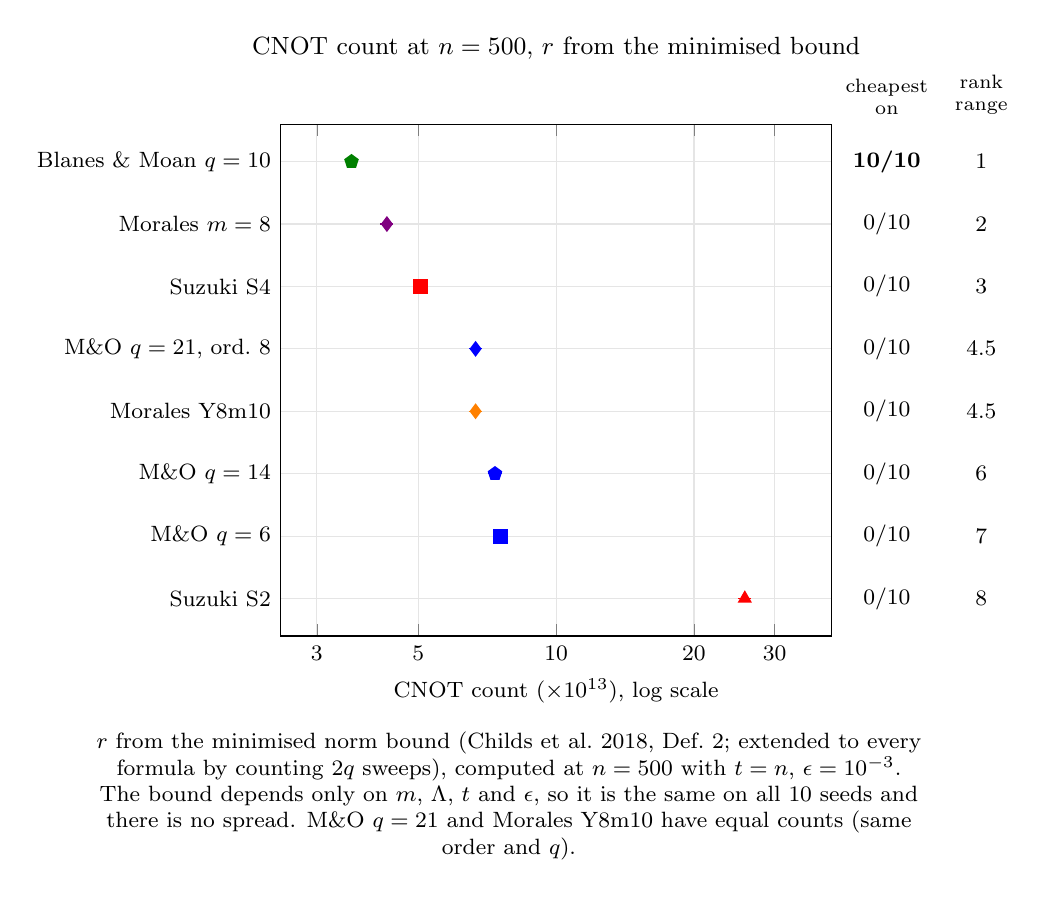
\begin{tikzpicture}
  \begin{semilogxaxis}[
    scale only axis, clip=false,
    at={(0cm,0cm)}, anchor=south west,
    width=7.0cm, height=6.5cm,
    title={CNOT count at $n = 500$, $r$ from the minimised bound}, title style={font=\small, yshift=14pt},
    xlabel={CNOT count ($\times 10^{13}$), log scale}, xlabel style={font=\footnotesize},
    xmin=2.5e+13, xmax=4e+14, xtick={3e+13,5e+13,1e+14,2e+14,3e+14}, xticklabels={3,5,10,20,30},
    xminorticks=false,
    y dir=reverse, ymin=0.4, ymax=8.6, ytick={1,2,3,4,5,6,7,8},
    yticklabels={{Blanes \& Moan $q=10$},{Morales $m=8$},{Suzuki S4},{M\&O $q=21$, ord.~8},{Morales Y8m10},{M\&O $q=14$},{M\&O $q=6$},{Suzuki S2}},
    tick label style={font=\footnotesize}, ytick style={draw=none},
    xmajorgrids=true, ymajorgrids=true, grid style={black!10},
  ]
    % bm-q10: plotted 3.57103e+13, seeds 3.57103e+13..3.57103e+13, cheapest on 10/10, rank 1..1
    \addplot[green!50!black, only marks, mark=pentagon*, mark size=2.4pt, mark options={solid, fill=green!50!black, line width=0.6pt}, error bars/.cd, x dir=both, x explicit, error bar style={solid, line width=0.6pt}] coordinates {
      (3.57103e+13,1) += (0,0) -= (0,0)
    };
    % morales-m8: plotted 4.26685e+13, seeds 4.26685e+13..4.26685e+13, cheapest on 0/10, rank 2..2
    \addplot[violet, only marks, mark=diamond*, mark size=2.4pt, mark options={solid, fill=violet, line width=0.6pt}, error bars/.cd, x dir=both, x explicit, error bar style={solid, line width=0.6pt}] coordinates {
      (4.26685e+13,2) += (0,0) -= (0,0)
    };
    % suzuki4: plotted 5.05115e+13, seeds 5.05115e+13..5.05115e+13, cheapest on 0/10, rank 3..3
    \addplot[red, only marks, mark=square*, mark size=2.4pt, mark options={solid, fill=red, line width=0.6pt}, error bars/.cd, x dir=both, x explicit, error bar style={solid, line width=0.6pt}] coordinates {
      (5.05115e+13,3) += (0,0) -= (0,0)
    };
    % mo-o8-q21: plotted 6.66564e+13, seeds 6.66564e+13..6.66564e+13, cheapest on 0/10, rank 4.5..4.5
    \addplot[blue, only marks, mark=diamond*, mark size=2.4pt, mark options={solid, fill=blue, line width=0.6pt}, error bars/.cd, x dir=both, x explicit, error bar style={solid, line width=0.6pt}] coordinates {
      (6.66564e+13,4) += (0,0) -= (0,0)
    };
    % morales-y8m10: plotted 6.66564e+13, seeds 6.66564e+13..6.66564e+13, cheapest on 0/10, rank 4.5..4.5
    \addplot[orange, only marks, mark=diamond*, mark size=2.4pt, mark options={solid, fill=orange, line width=0.6pt}, error bars/.cd, x dir=both, x explicit, error bar style={solid, line width=0.6pt}] coordinates {
      (6.66564e+13,5) += (0,0) -= (0,0)
    };
    % mo-q14: plotted 7.34983e+13, seeds 7.34983e+13..7.34983e+13, cheapest on 0/10, rank 6..6
    \addplot[blue, only marks, mark=pentagon*, mark size=2.4pt, mark options={solid, fill=blue, line width=0.6pt}, error bars/.cd, x dir=both, x explicit, error bar style={solid, line width=0.6pt}] coordinates {
      (7.34983e+13,6) += (0,0) -= (0,0)
    };
    % mo-q6: plotted 7.5521e+13, seeds 7.5521e+13..7.5521e+13, cheapest on 0/10, rank 7..7
    \addplot[blue, only marks, mark=square*, mark size=2.4pt, mark options={solid, fill=blue, line width=0.6pt}, error bars/.cd, x dir=both, x explicit, error bar style={solid, line width=0.6pt}] coordinates {
      (7.5521e+13,7) += (0,0) -= (0,0)
    };
    % suzuki2: plotted 2.58204e+14, seeds 2.58204e+14..2.58204e+14, cheapest on 0/10, rank 8..8
    \addplot[red, only marks, mark=triangle*, mark size=2.4pt, mark options={solid, fill=red, line width=0.6pt}, error bars/.cd, x dir=both, x explicit, error bar style={solid, line width=0.6pt}] coordinates {
      (2.58204e+14,8) += (0,0) -= (0,0)
    };
    \node[anchor=south, font=\scriptsize, align=center] at ([xshift=0.7cm]axis cs:4e+14,0.4) {cheapest\\on};
    \node[anchor=south, font=\scriptsize, align=center] at ([xshift=1.9cm]axis cs:4e+14,0.4) {rank\\range};
    \node[font=\footnotesize\bfseries] at ([xshift=0.7cm]axis cs:4e+14,1) {10/10};
    \node[font=\footnotesize] at ([xshift=1.9cm]axis cs:4e+14,1) {1};
    \node[font=\footnotesize] at ([xshift=0.7cm]axis cs:4e+14,2) {0/10};
    \node[font=\footnotesize] at ([xshift=1.9cm]axis cs:4e+14,2) {2};
    \node[font=\footnotesize] at ([xshift=0.7cm]axis cs:4e+14,3) {0/10};
    \node[font=\footnotesize] at ([xshift=1.9cm]axis cs:4e+14,3) {3};
    \node[font=\footnotesize] at ([xshift=0.7cm]axis cs:4e+14,4) {0/10};
    \node[font=\footnotesize] at ([xshift=1.9cm]axis cs:4e+14,4) {4.5};
    \node[font=\footnotesize] at ([xshift=0.7cm]axis cs:4e+14,5) {0/10};
    \node[font=\footnotesize] at ([xshift=1.9cm]axis cs:4e+14,5) {4.5};
    \node[font=\footnotesize] at ([xshift=0.7cm]axis cs:4e+14,6) {0/10};
    \node[font=\footnotesize] at ([xshift=1.9cm]axis cs:4e+14,6) {6};
    \node[font=\footnotesize] at ([xshift=0.7cm]axis cs:4e+14,7) {0/10};
    \node[font=\footnotesize] at ([xshift=1.9cm]axis cs:4e+14,7) {7};
    \node[font=\footnotesize] at ([xshift=0.7cm]axis cs:4e+14,8) {0/10};
    \node[font=\footnotesize] at ([xshift=1.9cm]axis cs:4e+14,8) {8};
  \end{semilogxaxis}
  \node[anchor=north, text width=10.5cm, align=flush center, font=\footnotesize] at (2.9cm,-1.1cm) {$r$ from the minimised norm bound (Childs et al.\ 2018, Def.~2; extended to every formula by counting $2q$ sweeps), computed at $n = 500$ with $t = n$, $\epsilon = 10^{-3}$. The bound depends only on $m$, $\Lambda$, $t$ and $\epsilon$, so it is the same on all 10 seeds and there is no spread. M\&O $q=21$ and Morales Y8m10 have equal counts (same order and $q$).};
\end{tikzpicture}
